% !TeX spellcheck = <none>

\documentclass[]{article}
\usepackage[T1]{fontenc}

\usepackage{polski}
\usepackage[utf8]{inputenc}
\usepackage[polish]{babel}
\usepackage{textcomp}

\usepackage{graphicx}
\graphicspath{ {./images/} }

%opening
\title{Programowanie zaawansowane - projekt}
\author{Magdalena Czumak \\
Przemysław Matuszczak\\
Bartosz Sowiński\\
Norbert Sulżycki\\
}

\begin{document}

\maketitle



\section{Problem badawczy}
Problemem badawczym postawionym w niniejszej pracy jest prognoza obciążenia parkingu samochodowego umieszczonego w Birningham, UK (regresja). Dane wykorzystane w projekcie zostały zaczerpnięte ze strony\\ $https://archive.ics.uci.edu/ml/datasets/Parking+Birmingham$ (plik: $dataset.csv$ zawiera wszystkie dane na temat wszystkich paringów). Ze wskazanych danych zostały wydzielone dotyczące tylko jednego prakingu $BHMBCCMKT01$ jako osobny plik (plik: $dataset-parking.csv$), następnie wydzielone zostały wszystkie dane dotyczące sobót dla tego parkingu (plik: $dataset-soboty.csv$).

\section{Model}
Modele zostały zbudowane przy wykorzystaniu algorytmu Drzewa Decyzyjnego ($https://scikit-learn.org/stable/auto_examples/tree/plot_tree_regression.html$). Kod dla obu modeli jest dostępny jako dwa osobne algorytmy (plik: $modelowanie.py$ oraz $parking.py$).\\
\\
Pierwszy wykres sporządzony został na podstawie wszystkich możliwych danych, które były dostępne. Zaobserwować można fakt, że jest on stosunkowo płaski i zdecydowanie mniej zróżnicowany niż posiadane dane (przy obu parametrach $n\_estimators$). Parametr $n\_estimators$ świadczy o tym, na ile części dane są dzielone, a następnie algorytm z każdej takiej pojedynczej części oblicza regresję liniową. Oznacza to, że im mniejsza wartość $n\_estimators$, tym na mniej części dane są dzielone.\\
\\
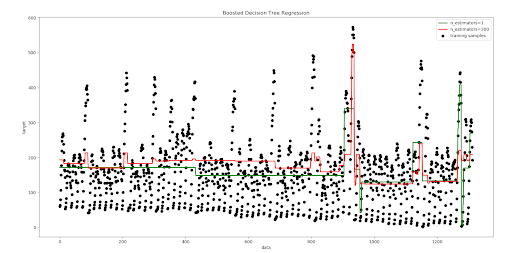
\includegraphics[width=12cm]{image-0}\\
\\
Kolejnymi zbudowanymi modelami (dla dwóch wartości $n\_estimators$) są widoczne na poniższym wykresie linie zielona i czerwona. Zbudowane one zostały na podstawie tylko i wyłącznie dostępnych danych z sobót. \\
\\
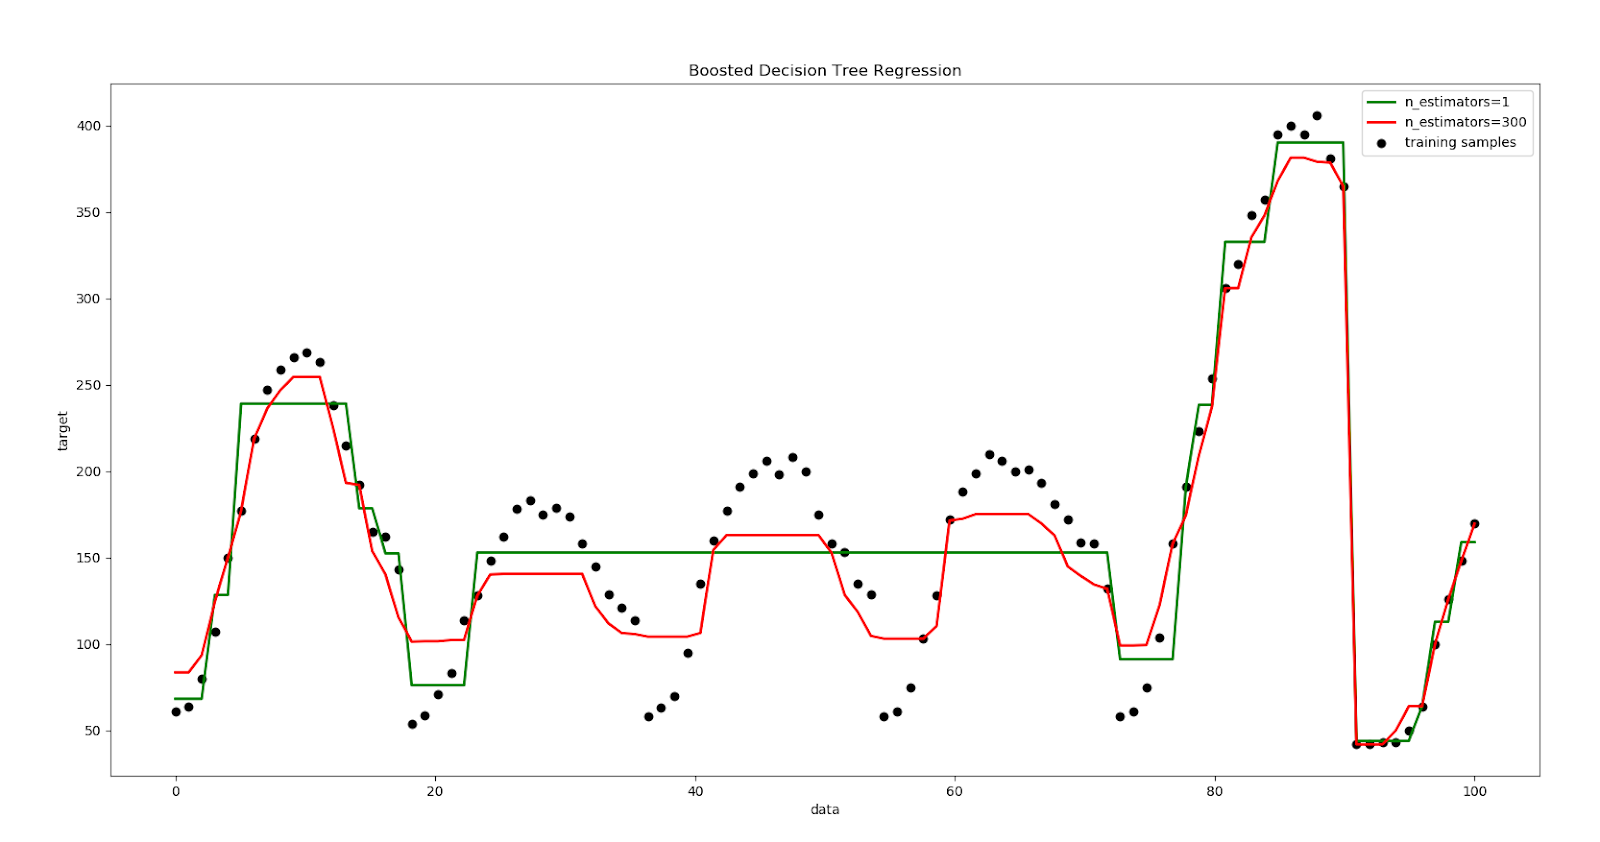
\includegraphics[width=12cm]{image-1}\\
\\
\section{Analiza porównawcza}
Zbudowanie powyższych modeli przy użyciu Drzewa decyzyjnego nie było trafnym pomysłem. Nie nadaje się ono do rozwiązania postawionego problemu, czyli prognozy przyszłego obciążenia parkingu. Aby możliwa była predykcja, koniecznym byłoby poznanie funkcji będącej modelem danych. W tym przypadku takowych modeli jest wiele funkcji (osobno dla każdego przedziału determinowanego przez parametr $n\_estimator$) .\\
\\
Jednakże warto wspomnieć inną cechę wspomnianego parametru. W przypadku mocno zróżnicowanych danych, na które wpływ miały różne szumy, zmniejszając $n\_estimators$, zmniejszamy jednocześnie wrażliwość modelu na zakłócenia. Zjawisko to jest zdecydowanie uwidocznione w przypadku pierwszego modelu, gdzie mimo dużego zróżnicowania danych, modele są wypłaszczone.

\section{Podsumowanie}
Podsumowując, zastosowanie Drzewa decyzyjnego nie nadaje się do tworzenia prognozy.


\section{Podział zadań}

\begin{itemize}
	\item Analiza problemu i przygotowanie danych wejściowych 
	\begin{itemize}
		\item Magdalena Czumak 
		\item Przemysław Matuszczak		
		\item Bartosz Sowiński
		\item Norbert Sulżycki
	\end{itemize}
	\item Przygotowanie danych dla modeli 
	\begin{itemize}
		\item Magdalena Czumak 
		\item Norbert Sulżycki
	\end{itemize}
	\item Tworzenie kodu Python
	\begin{itemize}
		\item Magdalena Czumak 
		\item Przemysław Matuszczak		
		\item Bartosz Sowiński
		\item Norbert Sulżycki
	\end{itemize}
	\item Analiza danych wynikowych
	\begin{itemize}
		\item Magdalena Czumak 
		\item Bartosz Sowiński
	\end{itemize}
	\item Przygotowanie dokumentu LaTeX
	\begin{itemize}
		\item Przemysław Matuszczak		
		\item Norbert Sulżycki
	\end{itemize}
\end{itemize}

\end{document}
